\documentclass{article}
\usepackage{graphicx} % Required for inserting images

\usepackage[utf8]{inputenc}
\usepackage[T1]{fontenc}


\usepackage{amsmath}
\usepackage{amssymb}						
\usepackage{amsthm}								

\usepackage{float} % to use the option H when include image

\usepackage{breakurl} % to break long line url

\usepackage{microtype}
\DisableLigatures{} % print -- instead of long dash


\usepackage{color}
\usepackage{listings} % Insert code block with highlight for specific language

\definecolor{dkgreen}{rgb}{0,0.6,0}
\definecolor{gray}{rgb}{0.5,0.5,0.5}
\definecolor{mauve}{rgb}{0.58,0,0.82}

\lstset{frame=tb,
	aboveskip=3mm,
	belowskip=3mm,
	showstringspaces=false,
	columns=flexible,
	basicstyle={\small\ttfamily},
	numbers=none,
	numberstyle=\tiny\color{gray},
	keywordstyle=\color{blue},
	commentstyle=\color{dkgreen},
	stringstyle=\color{mauve},
	breaklines=true,
	breakatwhitespace=true,
	tabsize=4
}

% Format page
\usepackage[a4paper,width=150mm,top=20mm,bottom=25mm]{geometry}

%\usepackage[a4paper,top=2.5cm,bottom=2cm,inner=3cm,outer=2cm,footskip=1cm]{geometry}
%\usepackage[left=2cm,right=2cm,top=2cm,bottom=2cm]{geometry}

\usepackage{url}
\usepackage{hyperref}
\hypersetup{
	colorlinks	= true,	%Colors links instead of ugly boxes
	breaklinks	= true,
	urlcolor	= blue,	%Color for external hyperlinks
	linkcolor	= blue,	%Color of internal links
	citecolor	= red	%Color of citations
}


% Comment with color
\newcommand{\hung}[1]{{\color{red} #1}}


\theoremstyle{plain}
\newtheorem{theorem}{Theorem}[section]
\newtheorem{conjecture}[theorem]{Conjecture}
\newtheorem{lemma}[theorem]{Lemma}
\newtheorem{proposition}[theorem]{Proposition}
\newtheorem{corollary}[theorem]{Corollary}
\newtheorem{problem}{Problem}
\newtheorem{question}{Question}

\newtheorem{theoremx}{Theorem}
\newtheorem{conjecturex}[theoremx]{Conjecture}
\renewcommand{\thetheoremx}{\Alph{theoremx}} % "letter-numbered" theorems

\theoremstyle{definition}
\newtheorem{definition}[theorem]{Definition}
\newtheorem{example}[theorem]{Example}
\newtheorem{notation}[theorem]{Notation}
\newtheorem{remark}{Remark}

\numberwithin{equation}{section}


\setcounter{tocdepth}{3}
%\setcounter{section}{0}
\parskip 3pt

\title{Security analysis of Bluetooth Low Energy Over-The-Air firmware updates}
\author{Huy Hung LE\\[0.5cm]{\small Supervisors: Aur\'elien Francillon and Romain Cayre}}
\date{June 29, 2023}
\begin{document}
\maketitle
\tableofcontents

\section*{Introduction}
\addcontentsline{toc}{section}{Introduction}

Device Firmware Update (DFU)  Over-The-Air (OTA) is a process that allow to update firmware running on a device over a Bluetooth Low Energy (BLE) connection from a smartphone or a computer. Nordic Semiconductor provides a proprietary DFU process which implemented in many smartwatches and smartlocks as a BLE Generic Attribute (GATT) Service (see Section \ref{gatt}). The chip that are widely used are nRF51 and nRF52 (see Section \ref{dk}). This project goal is to reverse engineer this DFU OTA process and identify potential vulnerabilities.

In Section \ref{preliminaries}, we will describe the Development Kits (DK) nRF51 and nRF52 (Section \ref{dk}), the Software Development Kits (SDK) (Section \ref{sdk}) and an overview of a GATT Service (Section \ref{gatt}).

In Section \ref{dfu}, we will describe the process of doing DFU over BLE. We give some remarks about the problems may encountered when doing DFU on the DKs: Remark \ref{gcc-latest}, \ref{nrfjprog}, \ref{old-nrfutil}, \ref{create firmware}, \ref{recommnd android}.

In Section \ref{reverse firmware packets}, we will describe in detail the content of a firmware packet.

In Section \ref{reverse dfu}, we will describe how we reverse the DFU process: capture the packets OTA (Section \ref{capture packages}), the detail of DFU protocol (Section \ref{protocol dfu open} and Section \ref{protocol dfu secure}). Then we redo the DFU process by writing a python program (Section \ref{python application}). We also gather some information about the process of validating a firmware packages in Section \ref{validate}. Section \ref{discover} can be consider as an application of Section \ref{python application}. It will be useful when we discuss about the security in Section \ref{security}.

Section \ref{security} contains all the important result related to security of the DFU process.

Finally, I would like to thank my supervisors Aur\'elien Francillon and Romain Cayre. I would not able to finish this project without them. I also learn a lot of interesting stuffs when doing this project: how to reverse engineering a protocol, understanding BLE, experiment with DKs, using tools and fixes the problems,...

\section{Preliminaries}\label{preliminaries}
In this section, we will describe the DKs (Section \ref{dk}), SDKs (Section \ref{sdk}) which are used in this project. We also give a few works on GATT Services of BLE in Section \ref{gatt}.
\subsection{Development kit}\label{dk}
In this project, we will use two DKs from Nordic Semiconductor:
\begin{itemize}
	\item nRF51, see \url{https://www.nordicsemi.com/Products/Development-hardware/nrf51-dk}.
	
	
\item nRF52, see \url{https://www.nordicsemi.com/Products/Development-hardware/nrf52-dk}.
\end{itemize}
The table below shows the relation between DKs, PCA numbers and chips.
\begin{figure}[H]
	\centering
	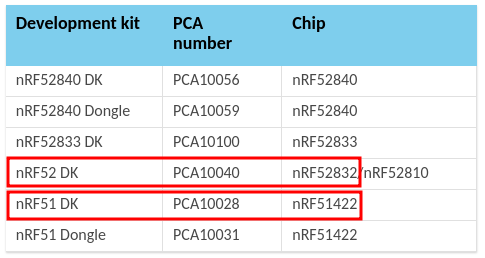
\includegraphics[width=0.7\linewidth]{images/DK-PCA-chip}
	\caption{Relation between development kits, PCA numbers, and chips\\
	\centering Source: \url{https://infocenter.nordicsemi.com/topic/ug_gsg_ses/UG/gsg/chips_and_sds.html}}	
	\label{fig:dk-pca-chip}
\end{figure}
\begin{remark}
	 The PCA number will be encountered a lot when we explore the software development kits: pca10028 for the nrf51 and pca10040 for nrf52.
\end{remark}

\subsection{Software development kit} \label{sdk}

The SDKs used are the nRF5 SDK, range from SDK v9.0.0 (2015) to v17.1.0 (2021). From now on, we will refer to them simply as "SDK". They can be downloaded at \url{https://www.nordicsemi.com/Products/Development-software/nRF5-SDK/Download?lang=en#infotabs}.

\begin{remark}
	Here is some further information about SDKs:
	\begin{itemize}
		\item The SDK v9.0.0 and v10.0.0 are called nRF51 SDK.
		\item The SDK v12.3.0 is the latest version that support nRF51.
		\item We can only download the SDK v7.0.0 and from v9.0.0 to v17.1.0. The structure of SDK v7.2.0 is a bit different. Consequently, SDK v7.2.0 and earlier version are not subjected to analysis in this project.
		\item Currently the nRF5 SDK is in maintenance mode. Nordic Semiconductor recommend the nRF Connect SDK (\cite{nrf-connect-sdk}).
	\end{itemize}
\end{remark}


\subsection{Generic Attribute Service} \label{gatt}
In this section, we will provide a short overview of the Generic Attribute Profile (GATT) of BLE (for more details, see \cite[chapter 4]{ble1},\cite[chapter 13]{ble2}):
\begin{itemize}
	\item BLE also known as Bluetooth Smart started as part of the Bluetooth Core Specification version 4.0 (see \cite{core}). It is aimed at "ultra" low power devices.
	\item The GATT within BLE defines how to manage and exchange data between BLE devices.
	\item Within the GATT, there are services. Each service contains its own set of characteristics. These characteristics consist of attributes.
	\item Attribute is the smallest data entities defined by the GATT. Some common attributes are handle (16 bits), type (UUIDs), permissions, value (can be UUIDs or anything), descriptors,$\ldots$
\end{itemize}
The DFU process is implemented as a BLE GATT service and a set of associated characteristics. We will discuss more about the DFU process and its corresponding GATT service in Chapter \ref{dfu} and Chapter \ref{reverse dfu}. Also see Section \ref{discover} to know the  implemented services and characteristics.

\section{Device Firmware Update process}\label{dfu}

A Softdevice is a precompiled and linked binary software implementing a wireless protocol developed by Nordic Semiconductor.

Device Firmware Update is the process of update the SoftDevice, bootloader, application or its combination on a device called the DFU target (for example, DK nRF51 and DK nRF52).\\
The new SoftDevice, bootloader, or application image can be transferred over-the-air (OTA) using the Nordic BLE DFU Service by a device called the DFU controller (for example, Android phone, Apple phone, laptop,...)

There are two main generation of the DFU process: The DFU process with open bootloader (SDK v11.0.0 and earlier) and the DFU process with secure bootloader (SDK v12.1.0 and later).

In this section, we will describe some main steps to do the DFU process and have some remarks.

\subsection{Compiling and flashing files from SDK to the DK}
In the gitlab repository (\cite{gitlab}) of this project, we have some compiled files from each SDK version. We also have some Makefile files to have easier to flashing files.

Some SDKs also provide pre-compiled files to flash to the DKs. In this section, we will explain the process of compiling and flashing files without using the pre-compiled from SDKs.
\subsubsection{Compiling files}
We will use \texttt{gcc-arm-none-eabi} as a compiler to compile program in the SDK. Each SDK version will need a specific version of \texttt{gcc-arm-none-eabi}. In this project, we use the extract version of \texttt{gcc-arm-none-eabi} for each SDK version. See Remark \ref{gcc-latest} if we want to use the latest version.


Below is the main steps to compile a program. Skip step 2 and 3 if we want to flash \texttt{open bootloader}.

1. Modify the file \path{<SDK-folder>/components/toolchain/gcc/Makefile.posix}. Here is an example of the original content of this file:
\begin{lstlisting}{language = Tex}
GNU_INSTALL_ROOT := /usr/bin/gcc-arm-none-eabi-4_8-2014q1
GNU_VERSION := 4.8.3
GNU_PREFIX := arm-none-eabi
\end{lstlisting}
We modify the first line: replace \path{/usr/bin} by the path to the extracted folder of \texttt{gcc-arm-none-eabi} after downloading.

2. Install \texttt{micro-ecc}:
\begin{lstlisting}{language = bash}
cd <SDK-folder>/external/micro-ecc
git clone https://github.com/kmackay/micro-ecc.git .
\end{lstlisting}
Then go to each folder \path{nrf52hf_armgcc/armgcc} and \path{nrf52nf_armgcc/armgcc}, run \texttt{make}.

3. Create a pair of public key and private key using \texttt{nrfutil} (\url{https://infocenter.nordicsemi.com/topic/sdk_nrf5_v17.1.0/lib_bootloader_dfu_keys.html}).\\
Store public key in a file named \path{dfu\_public\_key.c}. We replace the old file \path{dfu_public_key.c} in the SDK with the newly created file. The old file often is in the folder:
\begin{itemize}
	\item SDK v12.3.0 and earlier: \path{<SDK-folder>/examples/dfu/bootloader_secure/}
	\item SDK v13.0.0-v14.2.0: \path{<SDK-folder>/examples/dfu/dfu_req_handling}
	\item SDK v15.0.0-v17.1.0: \path{<SDK-folder>/examples/dfu/}
\end{itemize}
The private key \texttt{*.pem} will be use later when we create signed firmware packages.

4. Now, we have setup the requirement to compile the bootloader or application that we want in the SDK: Go to the folder of an example, choose the correct pca number (see Figure \ref{fig:dk-pca-chip}): pca10028 for nrf51 and pca10040 for nrf52, go to the folder armgcc and run \texttt{make}.


\begin{remark}\label{gcc-latest}
	We can use the latest version of gcc-arm-none-eabi. However we need some additional actions when compiling a program:
	\begin{itemize}
		\item In step 1, we need to modify the version in second line to be the latest version. For the path, modify all the path (not only \path{/usr/bin}) to match the path of the binary file of the latest version.
		\item In step 4, we need to search and remove the option \texttt{-Werror} in the \texttt{Makefile} before running \texttt{make}.
	\end{itemize}
\end{remark}
\subsubsection{Flashing files}
There are two ways:
\begin{itemize}
	\item When connect the board to the laptop, the board will appear as a folder name JLINK. We can simply copy the hex file to this folder to flash this file to the board.
	\item The second way is to use \texttt{nrfjprog}. In this project, we use this ways to flash files to the board.
\end{itemize}
\begin{remark}\label{nrfjprog}
	About using \texttt{nrfjprog}, if we see the Makefile from the SDK, some SDK use different options such as --reset, --sectorerase. Some options works with a SDK but not with other SDKs. For better experience, we recommend:
	\begin{itemize}
		\item Use --reset option in a separate command
		\item Do not use the option --sectorerase. Instead, we erase the board first then flash the file.
	\end{itemize}
\end{remark}


\subsection{Creating firmware packets}
To create a firmware packets, we need to use \texttt{nrfutil}, available at \url{https://www.nordicsemi.com/Products/Development-tools/nrf-util}. Some SDKs also provide pre-created firmware packages to test.

\begin{remark}\label{old-nrfutil}
	$ \bullet $ 
	To create firmware packages for doing DFU on board with open bootloader, we need to use a very old version of \texttt{nrfutil} (v0.5.1) which is a little bit tricky to find and install.
	
	$ \bullet $	We will refer old-nrfutil to this very old version of nrfutil and the newer version is simply called nrfutil.
	
	$ \bullet $	Below we explain the steps to install the old-nrfutil.
	
	First we need to create a python environment with python version 2.7. We use Conda to do this. Suppose that the name of the environment is py27:
	\begin{lstlisting}
conda create --name py27 python=2.7
	\end{lstlisting}
	Then we activate the python2.7 environment:
	\begin{lstlisting}
conda activate py27
	\end{lstlisting}
	Select a folder to clone the repository of pc-nrfutil (Public archive) and checkout a branch named \texttt{0\_5\_1}:
	\begin{lstlisting}
git clone https://github.com/NordicSemiconductor/pc-nrfutil .
git checkout 0_5_1
	\end{lstlisting}
	The follow the instruction in this git branch to install old-nrfutil. The old-nrfutil only works when we activate the py27 environment. To deactivate this environment to use the new nrfutil, we run \texttt{conda deactivate}.
\end{remark}


\begin{remark}\label{create firmware}
	We have some observations when creating the firmware packages:
	
	$ \bullet $	For \texttt{open bootloader}, we only need to specify the version of application or bootloader or softdevice that we want to create the firmware. Other version information will be the default value if not specify.
	
	$ \bullet $	For \texttt{secure bootloader}, we must specify the option --hw-version (hardware version), --sd-req (softdevice required on the board). The hardware version is 51 or 52. The sd-req value is specific in the nrfutil tool when using --help option.
\end{remark}


\subsection{Doing the DFU process}
We can use nrfutil to do the DFU process from laptop via BLE, usb-serial,... However, in this project, we use an application named nrfConnect in Android or Iphone.

To do the DFU process, first, send the firmware that we created to smart phone device. Now, open the application nrfConnect and scan. After flashing files to the board, we should see the advertiser name "DfuTarg". Choose to do the DFU and select the firmware. It should show a table of data rate and the process doing DFU. When it reaches 100\%, the DFU should success.

\begin{remark}\label{recommnd android}
	 We recommend to use Android phone for some reasons:
	 \begin{itemize}
	 	\item the nrfConnect application on Android has more functionality than in Iphone.
	 	\item Android phone has the ability to record the bluetooth packets sent from it. It will be useful when we want to analysis the DFU protocol. Iphone may also have similar ability but we have not found yet. 
	 \end{itemize}
\end{remark}

\section{Reverse the firmware packets}\label{reverse firmware packets}
In this section, we describe the content of the firmware packet and see the difference between two cases: open bootloader and secure bootloader.

The firmware package is a zip file. We can use nrfutil to read a firmware packet create by nrfutil (not works with old-nrfutil).

\begin{figure}[H]
	\centering
	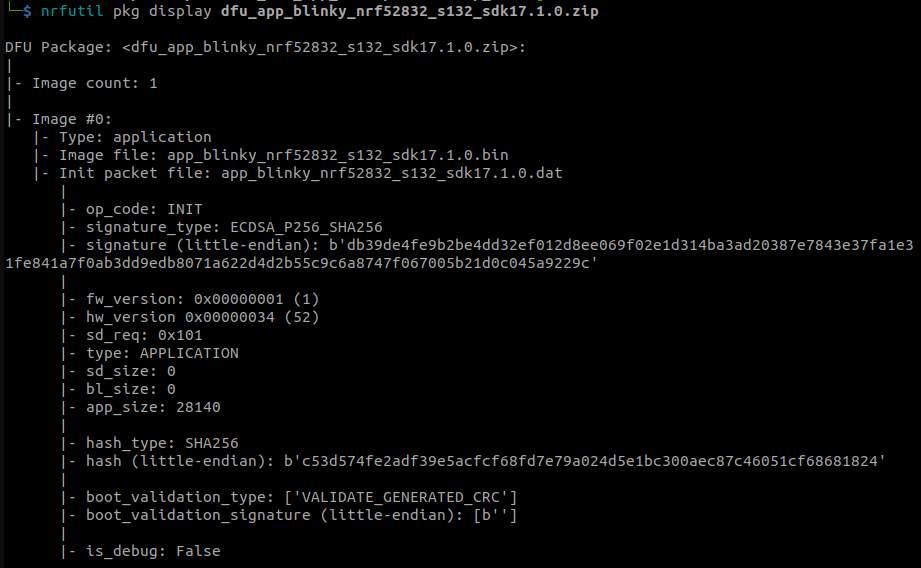
\includegraphics[width=0.7\linewidth]{images/nrfutil-view-zip}
	\caption{}
	\label{fig:nrfutil-view-zip}
\end{figure}


After extracting the package, we have three files: two files with same name but different extension \texttt{.dat}, \texttt{.bin} and a file \texttt{manifest.json}.

\subsection{File manifest.json}
Let us look at the files \path{manifest.json} in open bootloader case and secure bootloader case:
\begin{figure}[H]
	\centering
	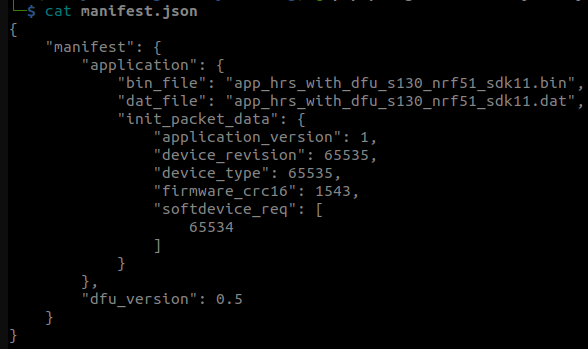
\includegraphics[width=0.7\linewidth]{images/manifest-open}
	\caption{manifest.json - open bootloader}
	\label{fig:manifest-open}
\end{figure}
\begin{figure}[H]
	\centering
	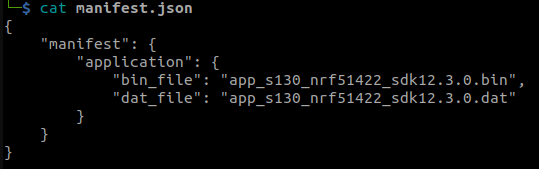
\includegraphics[width=0.7\linewidth]{images/manifest-secure}
	\caption{manifest.json - secure bootloader}
	\label{fig:manifest-secure}
\end{figure}
We can see that:
\begin{itemize}
	\item Both files has a key to indicate this is a firmware of an application. They also have the name of the \path{bin_file} and \path{dat_file} in this firmware.
	\item The open-bootloader file has more information about the firmware. Some values such as 65535 is the default value (when we do not specify these value during creating the firmware packets).
\end{itemize}
the open bootloader provide more detail about the firmware packages

\subsection{File .dat}
Let us look at the file \path{.dat}:

\begin{figure}[H]
	\centering
	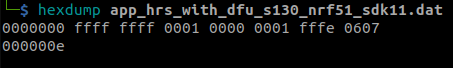
\includegraphics[width=0.7\linewidth]{images/dat-open}
	\caption{*.dat file - open bootloader}
	\label{fig:dat-open}
\end{figure}

\begin{figure}[H]
	\centering
	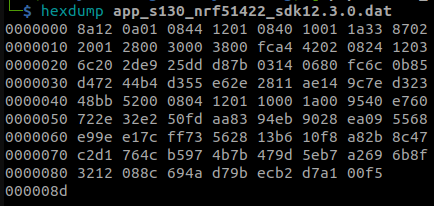
\includegraphics[width=0.7\linewidth]{images/dat-secure}
	\caption{*.dat file - secure bootloader}
	\label{fig:dat-secure}
\end{figure}
We can see that in case of open bootloader, the content of dat file is much more simpler than the case of secure bootloader.

\subsubsection{File .dat - open bootloader}\label{dat file open}
Now, by creating many firmware packages with different options values, we can identify the meaning of some part of this dat file. Let us recall some option in old-nrfutil
\begin{figure}[H]
	\centering
	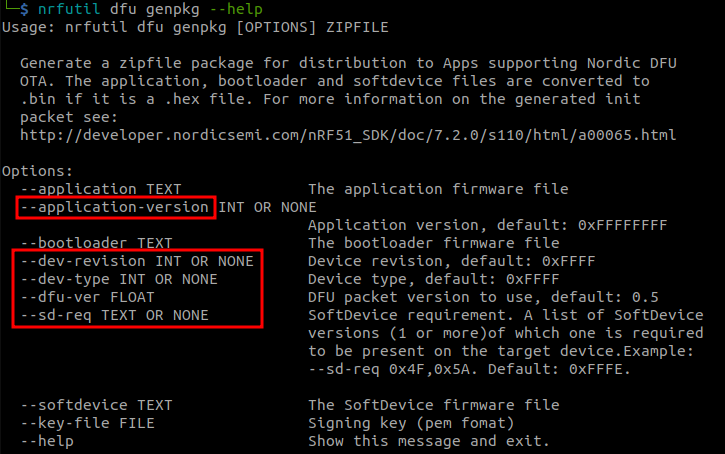
\includegraphics[width=0.7\linewidth]{images/old-nrfutil-options}
	\caption{Old-nrfutil options}
	\label{fig:old-nrfutil-options}
\end{figure}
Now, we create a firmware with all 5 options dev-type = 3, dev-revision = 4, application-version = 5, dfu-ver =6, sd-req = 7:
\begin{figure}[H]
	\centering
	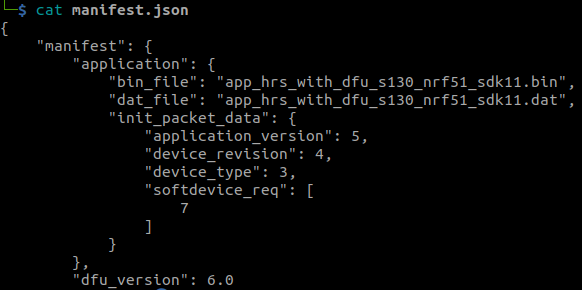
\includegraphics[width=0.7\linewidth]{images/dfu_type3revision4app5dfuver6sdreq7}
	\caption{dev-type = 3, dev-revision = 4, application-version = 5, dfu-ver =6, sd-req = 7}
	\label{fig:dfutype3revision4app5dfuver6sdreq7}
\end{figure}
\begin{figure}[H]
	\centering
	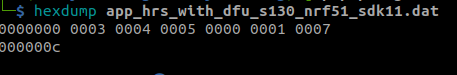
\includegraphics[width=0.7\linewidth]{images/dfu_type3revision4app5dfuver6sdreq7-dat}
	\caption{dev-type = 3, dev-revision = 4, application-version = 5, dfu-ver =6, sd-req = 7}
	\label{fig:dfutype3revision4app5dfuver6sdreq7-dat}
\end{figure}
We can see that: first two byte is dev-type, next is dev-revision, application-version. The next four bytes is unknown. The last two bytes is sd-req.

However, if we does not specify dfu-version: dfu-type = 3, dev-revision = 4, application-version = 5 , sd-req = 6:
\begin{figure}[H]
	\centering
	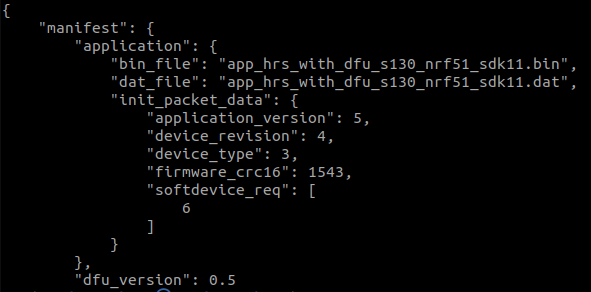
\includegraphics[width=0.7\linewidth]{images/dfu_type3revision4app5sd-req6-manifest}
	\caption{dfu-type = 3, dev-revision = 4, application-version = 5 , sd-req = 6}
	\label{fig:dfutype3revision4app5sd-req6-manifest}
\end{figure}
\begin{figure}[H]
	\centering
	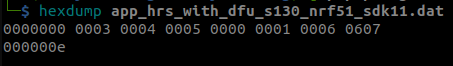
\includegraphics[width=0.7\linewidth]{images/dfu_type3revision4app5sd-req6-dat}
	\caption{dfu-type = 3, dev-revision = 4, application-version = 5 , sd-req = 6}
	\label{fig:dfutype3revision4app5sd-req6-dat}
\end{figure}
We can see that the last two bytes is CRC (0x0607=1543), two bytes before is the sd-req. The bytes 0000 0001 is unknown.

In conclusion, we guess that:
\begin{itemize}
	\item the first two bytes is the device type
	\item next two bytes is the device revision
	\item next two bytes is the application version
	\item next four bytes seems to be fixed: 0000 0001
	\item next two bytes is the softdevice required
	\item the dat file is 12 bytes or 14 bytes. If the dfu-version is specified, the dat file is only 12 bytes. If not, the dat file is 14 bytes and the last two bytes is CRC
\end{itemize}

\begin{remark}
	We also want to mention a link \url{https://infocenter.nordicsemi.com/topic/com.nordic.infocenter.sdk5.v11.0.0/bledfu_example_init.html}. This link explain the content of the init package (dat file): two bytes for device type, two bytes for device revision, but four bytes for the application verions, two bytes for supported softdevice, two bytes for checksum CRC-16-CCIT (which is optional). However, as we analyze above, it seems confused.
	
\end{remark}
\subsubsection{File .dat - secure bootloader}
By doing similar as above, we know some information from the file \path{.dat}:
\begin{figure}[H]
	\centering
	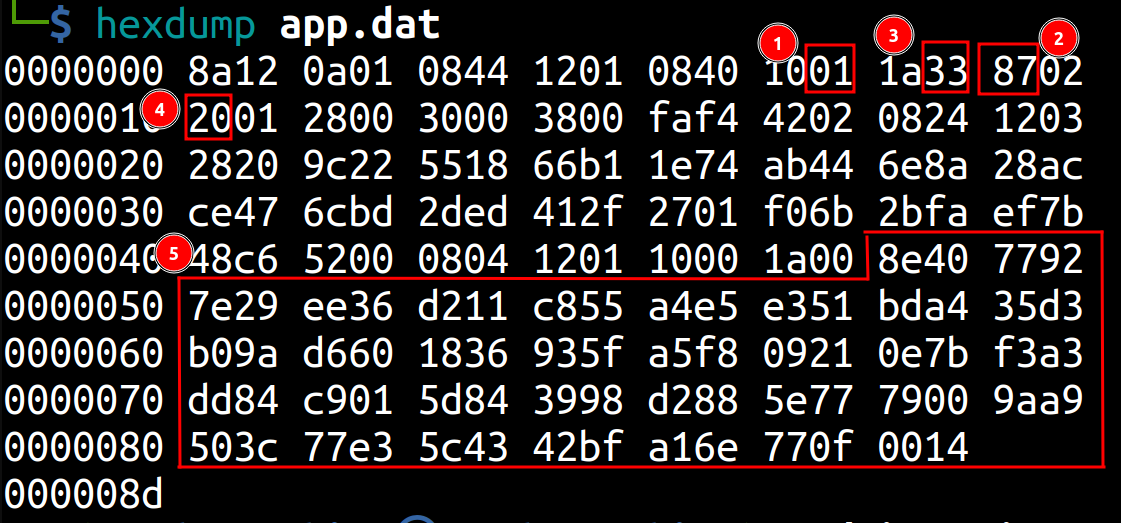
\includegraphics[width=0.7\linewidth]{images/reverse-dat-file-secure.png}
	\caption{Reverse dat file - secure bootloader}
	\label{fig:reverse-dat-secure}
\end{figure}

\begin{itemize}
	\item 1: application-version
	\item 2: sd-req
	\item 3+4 may related to hardware (we haven't check carefully)
	\item 5: signature of the hash.
\end{itemize}

\begin{remark}
	We can also see the information of a firmware zip file by nrfutil. But this only works for secure bootloader firmware packages.
	\begin{figure}[H]
		\centering
		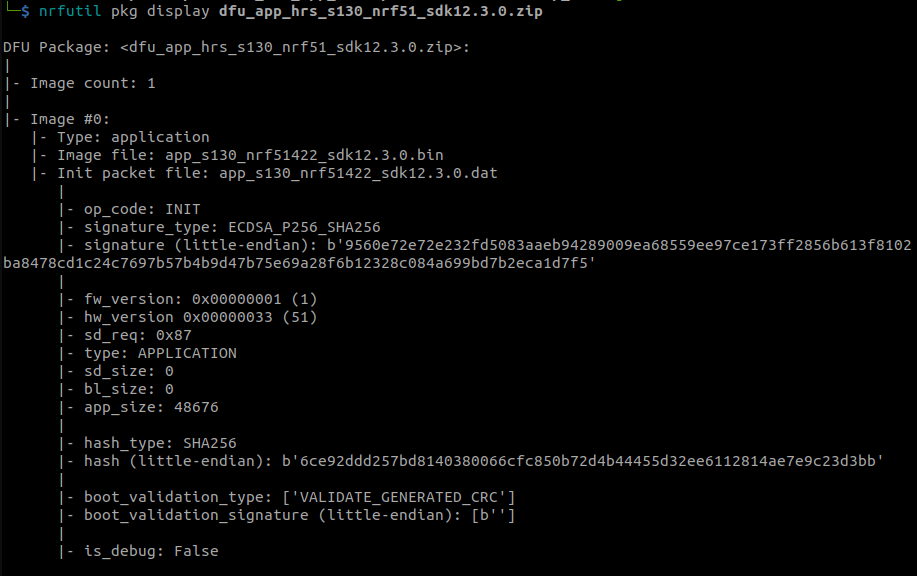
\includegraphics[width=1\linewidth]{images/nrfutil-see-information}
		\caption{}
		\label{fig:nrfutil-see-information}
	\end{figure}
\end{remark}
\subsection{File .bin}
This file is actually data of the hex file application, bootloader or softdevice.

\section{Reverse engineer DFU protocol}\label{reverse dfu}
A common method is to capture the file sent over the air then analyze all the data exchanged. We will explain how to sniff the data in Section \ref{capture packages} since it is not trivial with BLE. Then, we analyze the protocol in Section \ref{analyze packages}. And finally, in Section \ref{python application}, with the analyzing result, we write a python program to do the DFU process without application nrfConnect on smart phone.
\subsection{Captures the packages over the air}\label{capture packages}
There are two ways. However, the most stable way is using an Android phone.
\subsubsection{Captured the packets using Wireshark and another DK}
First we need another DK as an interface to capture the packet. We need to flash a specific firmware (nRF Sniffer) to the DK then configure Wireshark to be able to receive packets of the DFU process over the air. See \url{https://www.nordicsemi.com/Products/Development-tools/nrf-sniffer-for-bluetooth-le} for more details.

\begin{remark}
	It seems that we can use DK nrf52 to capture the DFU on nrf51 but not the inverse. The reason seems to relate to hardware support and compatibility.
\end{remark}
\subsubsection{Captured the packets using Android phone}
The folder and functionality may different between Android phone but the idea are the same. Here we use "Realme Narzo 50i Prime" phone.

First, turn off Bluetooth, then Enable Bluetooth HCI snoop log on Android phone. Then turn on Bluetooth and do the DFU process. After that, Disable Bluetooth HCI snoop log.

Now, we need to generate the log, we can choose "Bug report" in Android phone and wait for it to generate the report. The report will be stored in folder \path{/bugreports/} in Android phone. We can retrieve this zip file by using \texttt{adb pull}.

Another way to generate the log is to use \texttt{adb bugreport} in laptop. The log will be created in the current folder.

After generating the log, the log can be found in the zip file under the folder \path{FS/data/misc/bluetooth/logs/} with the name \path{btsnoop_hci.log}. This file can be viewed normally in Wireshark.

\subsection{Analyzing the captured packages}\label{analyze packages}

Fortunately, the SDK documentation has the information about the meaning of value sent through the air. However, it is not available in the latest SDK version. We have to find these information in some previous versions of SDK. We will not rewrite them here but provide the link for the information:

For open bootloader, these information mostly is in SDKv11.0.0 --> Examples --> DFU bootloader examples --> BLE\&HCI/UART Bootloader/DFU --> Transport layers. See
\url{https://infocenter.nordicsemi.com/topic/com.nordic.infocenter.sdk5.v11.0.0/bledfu_transport_bleservice.html}.


For secure bootloader, these information mostly is in SDKv12.3.0 --> Libraries --> Bootloader modules --> DFU transport --> BLE. See \url{https://infocenter.nordicsemi.com/topic/com.nordic.infocenter.sdk5.v12.3.0/lib_dfu_transport_ble.html}


Now we present the protocol of DFU on open bootloader and secure bootloader,
\subsubsection{DFU protocol - open bootloader} \label{protocol dfu open}

1. Trigger the DFU process: subscribe to descriptor of Legacy DFU Control Point.\\
2. Start DFU process 0x01 + firmware type: application, bootloader or softdevice.\\
3. Send length of softdevice, bootloader, application.\\
4. Initialize DFU parameter: send 0x02 00.\\
5. Send firmware dat file. It is also called init packet.\\
6. Initialize DFU parameter complete: send 0x02 01.\\
7. Set PRN (Packet receive notification) value to 10\\
8. Prepare to send firmware bin file: send 0x03.\\
9. Send the firmware bin file.\\
10. Ask to validate the firmware image: send 0x04.\\
11. Ask to activate the firmware image: send 0x05.

\subsubsection{DFU protocol - secure bootloader}\label{protocol dfu secure}


1. Trigger the DFU process: subscribe to descriptor of DFU Control Point.\\
2. Seclect Command Object.\\
3. Set PRN (Packet receive notification) value to 0.\\
4. Create Command Object with size of firmware dat file.\\
5. Send the firmware dat file.\\
6. Request to calculate CRC.\\
7. Request to execute the sent file.\\
8. Set PRN value to 10.\\
9. Send the firmware bin file. This step is more complicate than the other steps. See Remark \ref{send file}.


\begin{remark}\label{send file} The step of sending firmware bin file is different with the open bootloader case.
	In step 9 above, to send a large file greater than 4096 bytes, the process is as follows:\\
	1. Select last command object and create data object with size = 4096.\\
	2. Send this file as packets of 20 bytes data until 4096 bytes.\\
	3. Request to calculate CRC.\\
	4. Request to execute.\\
	5. Repeat from step 1 until send all the firmware bin file. For the last part of file which is smaller than <4096, the size in step 1 will be the size of this last part.
\end{remark}

\subsection{Validate the firmware}\label{validate}
The process of validating the firmware is documented in some SDK versions. This section is to gather those information to be able to analyze the security in Section \ref{security}.



\subsubsection{Validate the firmware - open bootloader}\label{sec check open}
The information is in  \url{https://infocenter.nordicsemi.com/topic/com.nordic.infocenter.sdk5.v11.0.0/bledfu_example_init.html}.

Procedure to validate the updated firmware image. The current implementation supports only CRC validation in addition to size validation (which is always performed). CRC validation is optional and uses the information provided in the Receive Init Data procedure.

The  implementation in SDK 11.0.0 includes checks for Device type and revision, Supported SoftDevices, and the checksum, but not for the Application version.

\begin{remark}\label{check open}
	As mentioned in the link, we can disable the check by not specific it when create firmware packages (hence, it will use default values such as  0xFFFF for device type and revision, 0xFFFE for softdevice)
\end{remark}
\subsubsection{Validate the firmware - secure bootloader} \label{sec check secure}
The information for validation is in:\\
SDK v12.3.0:  \url{https://infocenter.nordicsemi.com/index.jsp?topic=%2Fcom.nordic.infocenter.sdk5.v12.3.0%2Fble_sdk_app_dfu_bootloader.html&anchor=lib_bootloader_dfu_init}\\
SDK v17.1.0: \url{https://infocenter.nordicsemi.com/topic/sdk_nrf5_v17.1.0/lib_bootloader_dfu_validation.html}

In brieft, the validation process consists of pre-validation (after send the firmware dat file) and post-validation (after sending the firmware bin file).

Checking values: Hardware version, SoftDevice version, Firmware version, the hash of the packet, Signature of the packet, Available space (or Firmware size).


The order of checking may different between SDK versions.


The acceptance rules for versions:
\begin{itemize}
	\item Hardware version: need to match.
	\item Softdevice Firmware ID: need to match.
	\item Firmware version: some SDKs require ">", some SDKs require "$ \geq $".
\end{itemize}

\subsection{Using Python to do the DFU process}\label{python application}
With the information from Section \ref{protocol dfu open} and \ref{protocol dfu secure}, we were able to write a python program that can do the DFU process from laptop (see \cite[folder \path{dfu_by_python}]{gitlab}  for the latest version). Here we use a private framework name Whad-client (\cite{whad}) from Whad-team . It is developed by Romain Cayre and his team. It helps us easier in interacting with GATT server with action such as scanning, connecting, discovering, sending Write request, Write command,...

Our python program can do:
\begin{itemize}
	\item Scan for bluetooth devices, select a device in the list and connect to this device.
	\item Discover the services and characteristics of this device and print its attribute handle, UUIDs, name, value,...
	\item We also search the UUID in a database provided by NordicSemiconductor to get the corresponding name if it is available. The database is at \url{https://github.com/NordicSemiconductor/bluetooth-numbers-database}.
	\item The mtu default value is 23. We try to set another mtu value to see if it is support by the board.
	\item Read the firmware zip file, unzip it; choose the correct firmware dat file and bin file from the manifest.json file, calculate the sizes and send them.
\end{itemize}

\subsection{Services and Characteristics discovery - Open vs Secure bootloader}\label{discover}
We would like to devote this section to discuss about difference of the Services and Characteristics between open and secure bootloader. Here, we use the python program from Section \ref{python application}.


You can find in the end of this section some screenshots about GATT server when we run the python program to discover the device. Some differences are:
\begin{itemize}
	\item Name: The open bootloader has word "Legacy" in its name.
	\item UUIDs:\\
	Open bootloader: Service UUID start: with 0x1530; Characteristic UUID start with 0x1531.\\
	Secure bootloader: Service UUID has short form: 0xFE59.
	\item Open bootloader has extra Characteristic named "Legacy DFU Version" which readable.
\end{itemize}

\begin{figure}[H]
	\centering
	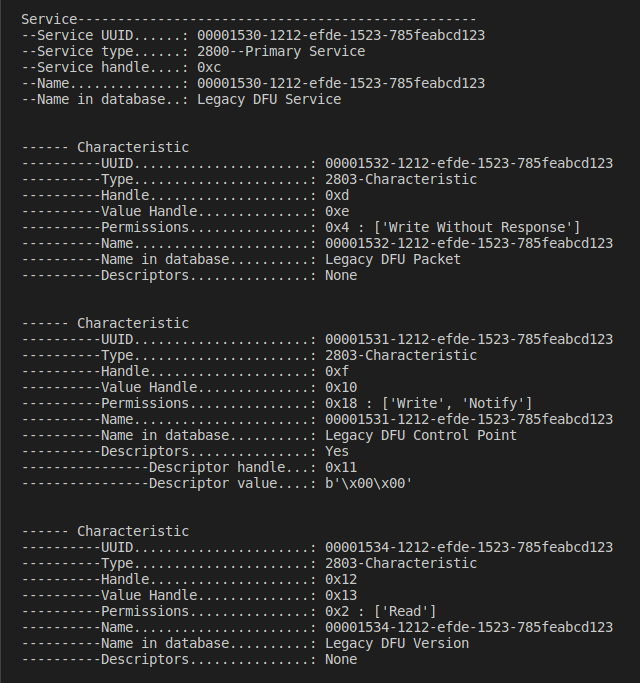
\includegraphics[width=0.7\linewidth]{images/gatt-open}
	\caption{GATT server - Open bootloader}
	\label{fig:gatt-open}
\end{figure}

\begin{figure}[H]
	\centering
	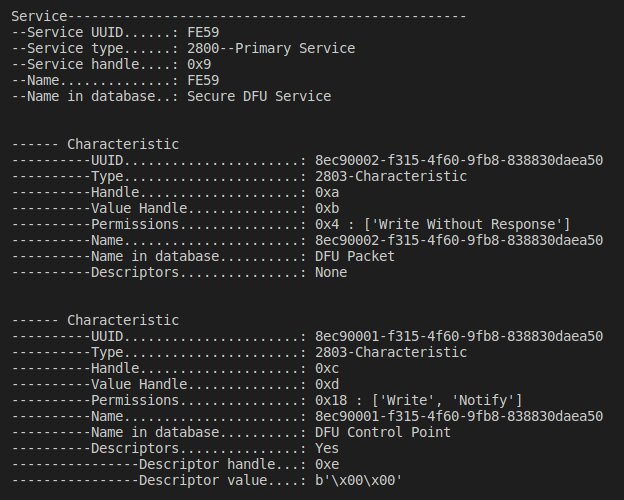
\includegraphics[width=0.7\linewidth]{images/gatt-secure}
	\caption{GATT server - Secure bootloader}
	\label{fig:gatt-secure}
\end{figure}


\section{Security analysis}\label{security}
In this section, we discuss the security of the DFU process:
\begin{itemize}
	\item By discovering Services and Characteristics name and UUIDs, we may know which kind of bootloader that the board using: open or secure. See Section \ref{discover}.
	\item By Remark \ref{send file}, we see that the DFU process on open bootloader may have a high change of corrupt since it only checks the CRC after finishing the sending. While in secure bootloader, for large file, it sends the data by small parts of 4096 bytes, request checksum, execute, then sends next part,...
	\item By  Section \ref{sec check open} and Remark \ref{check open}, we see some problems in the validation of the firmware package of open bootloader:
	
	With a legitimate firmware packages, an attacker can modify the dat file and manifest.json file, modify the check-required  values to the default values (see Section \ref{dat file open} to know where are the required values in the dat file so that the attacker can modify it correctly), then the validation will be skipped. The CRC algorithm is CRC-16-CCIT. The CRC checking algorithm is even optional and not implemented in some application.
	
	Hence, the attacker can craft a bad firmware package and pass the validation process.
	
	\item By Section \ref{sec check secure}, it seems difficult for an attacker to craft a bad firmware without the private key since the secure bootloader implements both CRC and signature validation.
	
	\item By Section \ref{sec check secure}, using the mechanism of validating firmware packages, if an attacker has access to a validated firmware package, the attacker can identify the version of hardware, softdevice that the target is using. The attacker does not need to do all the DFU process, just need to send the firmware dat file and see the response from the target. We can use the python application described in Section \ref{python application}.
\end{itemize}









\begin{thebibliography}{100}
%	\bibitem{example}	Authors.
%	\newblock {Name article}.
%	\newblock {\em Publisher}, paper, no, year.
	
	\bibitem{ble1} Townsend, K., Cuf, C., Akiba, \& Davidson, R. (2014). {\it Getting Started with Bluetooth Low Energy: Tools and Techniques for Low-Power Networking}. O'Reilly Media, Inc.\\
	\url{https://www.oreilly.com/library/view/getting-started-with/9781491900550/}
	
	
	\bibitem{ble2}Gupta, N. {\it Inside Bluetooth Low Energy}. (Artech House, 2016)\\ \url{https://us.artechhouse.com/Inside-Bluetooth-Low-Energy-Second-Edition-P1848.aspx}
	
	
	
	\bibitem{core} Bluetooth Core Specification 4.0, available at \url{https://www.bluetooth.com/specifications/specs/core-specification-4-0/}
	
	
	
	\bibitem{gitlab} Gitlab repository of the project:  \url{https://gitlab.eurecom.fr/lehh/spring2023-Security-analysis-of-Bluetooth-low-energy-Over-the-Air-firmware-updates}


	\bibitem{whad} Whad-client private project: \url{https://github.com/whad-team/whad-client}


	\bibitem{nrf-connect-sdk} nRF Connect SDK: \url{https://www.nordicsemi.com/Products/Development-software/nRF-Connect-SDK}
	
\end{thebibliography}


\end{document}
